\chapter{Active Directory Overview}

\begin{itemize}
    \item Active Directory Objects
    \item Active Directory Components
    \item Logical Structures
    \item Physical Structure
    \item Understanding Active Directory Concepts
    \item Domain Controller Installation
    \item Administering Active Directory
    \item Creating and Configuring Site Replication
    \item 

\end{itemize}

\subsection{Active Directory Objects and Attributes}

\begin{figure}
    \centering
    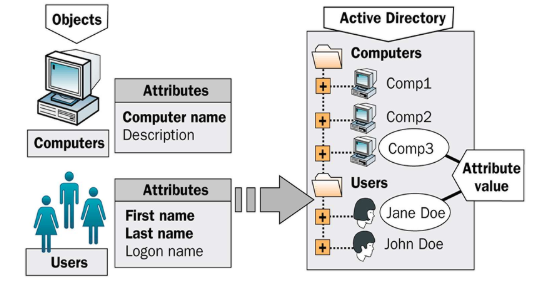
\includegraphics[width=1\linewidth]{adobj.png}
    \caption{FIGURE 1. Active Directory Objects and Attributes}
    \label{fig:placeholder}
\end{figure}

Active Directory Definitions

\begin{itemize}
    \item Resources stored in the directory, such as user data, printers, servers, databases, groups, computers, and security policies, are known as Objects.
    \item An object is a distinct named set of attributes that represent a network resource.
    \item Attributes are characteristics of objects in the directory.
    \item Objects are organized into classes, which are logical groupings of  objects.
    \item Objects are known as containers and can contain other objects.
\end{itemize}
Attributes and Classes

Attributes:

\begin{itemize}
    \item Defined separately from classes.
    \item Defined only once and can be used in multiple classes.
    \item Store the information that describes the object.
\end{itemize}
Classes:

\begin{itemize}
    \item Are collections of attributes.
    \item Describes the possible objects that can be created.
    \item Are also referred to as Object Classes.
    \item Every object is an instance of an object class.
\end{itemize}

Active Directory Components

\begin{itemize}
    \item Logical Structure
    \begin{itemize}
        \item Domains
        \item Organizational Units (OUs)
        \item Trees
        \item Forests
    \end{itemize}
    \item Physical Structure
    \begin{itemize}
        \item Sites
        \item Domain Controllers
    \end{itemize}
\end{itemize}

Logical Hierarchical Structure

Essential Terminology;l

\begin{itemize}
    \item \textbf{\textbf{Command Injection: }A type of security vulnerability where an attacker tricks an application into executing unintended operating system commands. It often results from improper input handling and insufficient access controls.}
    \item \textbf{\textbf{Active Directory (AD): }Microsoft’s centralized identity and access management directory services that governs user authentication, authorization, and policy enforcement across enterprise environments.}
    \item \textbf{\textbf{Remote Code Execution (RCE): }The unauthorized ability to run arbitrary code on a target machine from a remote location, often through exploits like command injection.}
    \item \textbf{\textbf{Least Privilege: }A foundational security principle where accounts and services are granted the minimal access necessary to perform their tasks. Limiting privileges reduces potential damage from compromise.}
    \item \textbf{\textbf{Privilege Escalation: }The process of exploiting a flaw to gain higher access rights than initially granted, often a goal of command injection attacks.}
\end{itemize}

\subsection{\textbf{Introduction to Command Injection Attacks}}

Command injection attacks are a class of security exploits where an attacker supplies malicious input to trick a web application into executing unintended commands on the underlying operating system. These attacks typically occur when user-supplied input is  not properly sanitized or is passed directly to shell interpreters or system APIs (Application Programming Interfaces). Unlike general input validation vulnerabilities, command injection specifically targets the interface between an application and the system-level execution environment.

In modern enterprise networks - particularly those reliant on Active Directory (AD) - command injection is especially dangerous. AD environments are dense with interconnected systems, administrative scripts, and automated processes that often execute with elevated privileges. A single vulnerable entry point, such as a poorly secured PowerShell script or an administrative web panel, can give attackers the foothold needed to move laterally, escalate privileges, and compromise domain controllers.

What makes command injection so potent is that it allows attackers to operate with the permissions of the vulnerable process. If that process runs with high-level privileges, the attacker gains immediate access to powerful system capabilities - ranging from creating user accounts to disabling security software mechanisms. Moreover, attackers frequently use these injections to chain together additional techniques, enabling persistence and full-blown Remote Code Execution (RCE).

The rise of automation tools, misconfigured scripts, and the complexity of AD environments has widened the attack surface for command injection. As a result, even organizations with mature security programs continue to be vulnerable. Understanding the mechanics of command injection is critical not only for offensive security professionals, but also for defenders tasked with securing core identity infrastructure.

To fully grasp why these attacks are so effective and impactful, it’s first essential to understand the backdrop in which they occur.

\subsection{Background: Active Directory Environments}

Active Directory is the backbone of authentication and access management in most enterprise Windows networks. It coordinates identities, permissions, and policies across user devices, servers, and services. AD organizes resources into forests, domains, and \textit{OUs (Organizational Units)}, enabling granular control. Its tight integration with Windows services and reliance on protocols like \textit{LDAP (Lightweight Directory Access Protocol)}, Kerberos, and \textit{SMB (Server Message Block)} makes it both powerful and complex. Misconfigurations or abuse of trusted systems within AD can have cascading effects on enterprise security.

AD’s centralized role means that any attack on it - especially through something as low-friction as command injection  can quickly escalate. Scripts and services commonly used in AD management, such as Group Policy Objects (GPO) update scripts or automated provisioning tools, often rely on system commands that, if manipulated, can yield domain-wide consequences.

\subsection{Architecture and Key Components}

AD is composed of various interdependent elements, such as:

\begin{itemize}
    \item \textbf{\textbf{Domain Controllers (DCs): }Central servers responsible for authenticating users, managing security policies, and maintaining a synchronized replica of the AD database.}
    \item \textbf{\textbf{Group Policy Objects (GPOs): }Mechanisms for enforcing system configurations script execution, and security rules across Organizational Units (OUs).}
    \item \textbf{\textbf{Organizational Units (OUs): }Containers used to logically structure AD objects like users, groups, and computers.}
    \item \textbf{\textbf{Security Principals: }Identifiable entries within AD - users, groups, and computers - that are subject to security policies.}
    \item \textbf{\textbf{Trust Relationships: }Logical links between domains that determine how authentication and access control are handled across different parts of the AD forest.}
\end{itemize}

Understanding how these components interact provides insight into how a single common injection vulnerability in one part of the system can ripple through the rest. For example, a malicious command injected into a script managed by GPOs could propagate to hundreds of machines with minimal visibility.

\subsection{Common Security Practices}

Defending an AD environment from injection and other attacks requires layered and disciplined security practices to be enforced and enabled, such as:

\begin{itemize}
    \item Implementing least privilege on all accounts and service roles
    \item Segmenting networks to reduce attack surfaces and exposure
    \item Maintaining a consistent patch cadence and update regiment for OS, applications, and middleware
    \item Enforcing multi-factor authentication on privileged accounts
    \item Using SIEM platforms for real-time threat detection
    \item Locking down PowerShell usage and scripting environments
    \item Employing application allowlisting to control executable code
\end{itemize}

While these practices reduce exposure, they are often inconsistently applied or bypassed through misconfigurations, poor visibility, or human error. That’s why attackers frequently turn to techniques like command injection - they exploit the blind spots and automation that defenders take for granted.

\subsection{Common Threat Landscape}

AD environments are prime targets for both opportunistic attackers and nation-state actors. Common threats include:

\begin{itemize}
    \item \textbf{\textbf{Insider Threats: }Employees or contractors abusing access}
    \item \textbf{\textbf{Credential Dumping: }Attackers extracting passwords and hashes from memory or registries}
    \item \textbf{\textbf{Misconfigured GPOs or User Rights: }Enabling privilege escalation or unintentional administrative access}
    \item \textbf{\textbf{Command and Control (C2) Implants: }Leveraging scripting and scheduling systems to maintain persistent access}
\end{itemize}

Many of these threats either originate from or leverage command injection techniques. For example, an attacker may use an initial injection to extract credentials, then use those credentials to move laterally using trusted administrative tools. The result is an attacker who looks like a legitimate user but operates with malicious intent - and usually with minimal detection.

\subsection{Command Injection Attacks: Foundational Elements}

Command injection attacks exploit weak input handling where user input is passed unsanitized into system-level functions. In AD environments, many services and automated scripts interact directly with the operating system - making these weak points especially dangerous. When a script running under elevated privileges accepts unvalidated input, an attacker can inject commands that execute with the full power of that script’s context.

\subsubsection{Command Injection Vulnerability Examples}

Here are three examples of how an application vulnerability can lead to command injection attacks. These examples are based on code provided by OWASP.

Example 1: File Name as Command Argument

This example highlights a program that allows remote users to view the contents of a file, without being able to modify or delete it. The program runs with root privileges:

\begin{table}
\centering

\begin{tabular}{| l |}
\hline
int main(char*argc, char**argv) \{char cmd[CMD\_MAX] = “/usr/bin/cat”;strcat(cmd, argv[1]);system(cmd);\} \\
\hline

\end{tabular}

\end{table}

Although the program is supposedly innocuous—it only enables read-only access to files—it enables a command injection attack. If the attacker passes, instead of a file name, a string like ; rm -rf /all. The call to system() will fail to execute, and then the operating system will perform recursive deletion of the root disk partition.

Example 2: Manipulating \textbf{\$APPHOME }Environment Variable

The following code snippet determines the installation directory of a certain application using the \$APPHOME environment variable and runs a script in that directory.

...

char* home=getenv("APPHOME");

char* cmd=(char*)malloc(strlen(home)+strlen(INITCMD));

if (cmd) \{

strcpy(cmd,home);

strcat(cmd,INITCMD);

execl(cmd, NULL);

\}

…

The problem is that the code does not validate the contents of the initialization script. If the attacker manages to modify the \$APPHOME variable to a different path, with a malicious version of the script, this code will run the malicious script. This constitutes a command injection attack.

Example 3: Manipulating \textbf{\$PATH} Variable

The following code may be used in a program that changes passwords on a server, and runs with root permissions:

\begin{table}
\centering

\begin{tabular}{| l |}
\hline
system(“cd /var/yp \&& make \&> /dev/null”); \\
\hline

\end{tabular}

\end{table}

The problematic part of this code is the use of make. While the attacker cannot change the code itself, because it does not accept user inputs, they can modify the \$PATH variable. This can cause the command to execute in a different path controlled by the attacker. In that other folder path, the attacker can plant a malicious version of the make binary.

Because the parent program has root privileges, the malicious version of make will now run with root privileges.

The bottom line of all three examples is that any command that invokes system-level functions like system() and exec() can lend their root privileges to other programs or commands that run within them.

\subsection{Command Injection Methods}

Here are some of the vulnerabilities that commonly lead to a command injection attack.

\subsubsection{Arbitrary Command Injection}

Some applications may enable users to run arbitrary commands, and run these commands as is to the underlying host.

\subsubsection{Arbitrary File Uploads}

If an application allows users to upload files with arbitrary file extensions, these files could include malicious commands. On most web servers, placing such files in the webroot will result in command injection.

\subsubsection{Insecure Serialization}

Server-side code is typically used to deserialize user inputs. If deserialization is performed without proper verification, it can result in command injection.

\subsubsection{Server-Side Template Injection (SSTI)}

Many web applications use server-side templates to generate dynamic HTML responses. This makes it possible for attackers to insert malicious server-side templates. SSTI occurs when user input is embedded in a template in an insecure manner, and code is executed remotely on the server.

\subsubsection{XML External Entity Injection (XXE)}

XXE occurs in applications that use a poorly-configured XML parser to parse user-controlled XML input. This vulnerability can cause exposure of sensitive data, \textit{Server-Side Request Forgery (SSRF)}, or denial of service attacks.

\subsection{Command Injection Prevention}

Here are several practices you can implement in order to prevent command injections:

1. Avoid system calls and user input—to prevent threat actors from inserting characters into the OS command.

2. Set up input validation—to prevent attacks like XSS and SQL Injection.

3. Create a white list—of possible inputs, to ensure the system accepts only pre-approved inputs.

4. Use only secure APIs—when executing system commands such as execFile()

5. Use execFile() securely—prevent users from gaining control over the name of the program. You should also map user input to command arguments in a way that ensures user input does not pass as-is into program execution.

Scope and Significance of Command Injection Attacks

This isn’t just a developer oversight; it’s a systemic threat. A single vulnerability can open the door to domain-wide consequences. Attackers can trigger scheduled tasks, manipulate Active Directory object properties, extract credentials, and modify Group Policy settings. These attacks are high-impact, low-effort when the right conditions are present.

Anatomy of a Command Injection Attack

1.>> Reconnaissance

Reconnaissance involves a careful look at your target before any actual movement takes place. The main goal is to gather as much information as possible about the system, network, or application. A key part of this phase is identifying potential targets that use Active Directory, which is a service that manages user accounts and permissions across many computer networks in organizations. Attackers often focus on AD-connected services because they hold sensitive data, and provide permissions and access control, which can easily be manipulated by an attacker with mal intent.

Attackers will search for web applications or services that interact with AD, such as login portals, company portals, or management tools. These apps often take user input like usernames, passwords, or other login details. Scripts or forms that process that input are prime targets. Attackers look for weak points in these scripts - for example, forms that don’t validate user input properly, or sites that run outdated software. Such vulnerabilities can be exploited to gain unauthorized access or gather user data.

Reconnaissance activities can often last months, and sometimes, years. This process usually begins by scanning the network for live hosts, open ports, and available services. Tools can help identify web servers hosting applications and scripts. For instance, an attacker might use a scanner to find login pages or admin panels that are not protected well. Beyond just finding the services, attackers seek out details like operating system builds and versions, which can reveal to the attacker known security flaws. Recognizing these weak spots that provide an entry into the network helps attackers to strategically plan their next move.

Understanding what kinds of services and scripts are present allows attackers to craft targeted attacks. For example, if they discover a web app that relies on a certain framework. If user inputs are taken through forms, they might test these inputs for vulnerabilities like injection or Cross-Site Scripting (XSS). Identifying and cataloging this information forms the foundation of the reconnaissance process, giving attackers the knowledge they need to proceed with further exploits.

In sum, reconnaissance is about gathering detailed information on targets, especially focusing on services linked with AD and user input points. This stage provides you a map of possible entry points, attack vectors and their weaknesses, making it an essential step in the attack chain for system exploitation. It requires patience and attention to detail, as knowing when and  what to attack depends heavily on what you discover during this initial pre-attack phase.

\textbf{2. Injection}

Injection is a common attack where an indivdual insert malicious shell commands into a website or application’s input fields. This happens when the system doesn’t properly check or filter user inputs, allowing harmful commands to slip through. When these commands are executed, they can give that individual control over the server or device, leading to data theft, corruption, or even complete system or domain takeover.

For example, imagine a website where you have to enter your username. If the site doesn’t validate the input (e.g., the password you just typed in), an attacker might enter a command like “; rm -rf /” in the username field. If the server executes this command without checking, or validating the user input, it could delete important files or harm the entire system. Harmful commands like these are called \textit{shell commands} because they instruct the operating system to perform specific actions.

Attackers look for vulnerabilities of this kind - where applications directly pass user inputs into a command line or script without performing any kind of sanitization check or validation that the command is legitimate. Manipulations of this kind often happen in chatbots, database queries, or any system that uses shell commands behind the scenes. They exploit these vulnerabilities to execute custom commands that shouldn’t be allowed, or that aren’t part of the original source code detailing the functionalities and capabilities of the coded software. Attackers might use injection to access sensitive data, change website content (webpage defacement is a popular attack that uses command injection practices), or cause the system to crash altogether.

Injection attacks are a major security concern for defenders. Studies show that injection flaws are among the most common ways attackers initially gain access to systems. When successful, these attacks can cause serious damage, from leaking private information to shutting down critical infrastructure, such as water and waste services, emergency and medical response services, among more. Protecting against injection involves thorough checking user inputs, escaping special characters, and avoiding dynamic command creation with untrusted data.

Understanding injection is crucial for keeping systems safe. By recognizing how malicious commands sneak into input paths, as an ethical hacker, you can build stronger defenses. You can recommend to developers to be cautious when handling user data and ensure their code doesn’t accept or execute harmful input. Proper security measures are essential to prevent attackers from turning simple input fields into gateways for harmful commands.

Understanding injection is crucial for keeping systems safe. By recognizing how malicious commands sneak into input paths, businesses can build stronger defenses. Developers need to be cautious when handling user data and ensure their code doesn’t accept or execute harmful input. Proper security measures are essential to prevent attackers from turning simple input fields into gateways for harmful commands.

\subsection{Mitigating Command Injection: Technical Controls and Best Practices for Defenders

}

Effective defense against command injection attacks begins with a disciplined approach to input handling and execution hygiene. Systems must assume that all external input is potentially hostile, and enforce strict validation, encoding, and safe execution strategies to neutralize risk.

\subsubsection{\textbf{1. Input Validation and Allowlisting}}

All user-supplied input should be validated against a strict allowlist of acceptable characters, formats, and values. Reject any input that does not conform to expected patterns, particularly in the context of command-line execution or administrative scripting. For example, the below is a PowerShell script that will validate user input for a username field:

\begin{table}
\centering

\begin{tabular}{| l |}
\hline
param([string]\$username)\textbf{if} (\$username -notmatch '\^[a-zA-Z0-9\_-]\{3,20\}$') \{

throw "Invalid input"

\} \\
\hline

\end{tabular}

\end{table}

This pattern explicitly allows only alphanumeric usernames with underscores or hyphens and a specific length range, reducing the chance of injection via name-based parameters.

\subsubsection{2. Escaping Special Characters}

When input must be used in contexts where escaping is required (e.g., shell commands, HTML, SQL), use encoding functions that neutralize control characters. For shell commands, escaping characters like \&, |, ;, >, and quotes are critical. Below is a script for escaping input written in Bash (Server-Side Scripting):

\begin{table}
\centering

\begin{tabular}{| l |}
\hline
user\_input=\$(printf ‘\%q’”\$1”)cmd=”ls -la /home/\$user\_input”eval”\$cmd” \\
\hline

\end{tabular}

\end{table}

This example uses an argument array instead of interpolating the \$user variable directly into a string, avoiding unintended execution flow.

\subsubsection{3. Avoid Dynamic Command Construction}

Dynamic construction of system or database commands using string concatenation invites injection. Instead, use native parameterization and safe APIs

Below is an unsafe PowerShell script (vulnerable):

\begin{table}
\centering

\begin{tabular}{| l |}
\hline
userInput = Read-Host "Enter username"

Invoke-Expression "Get-ADUser -Filter \{Name -eq '\$userInput'\} \\
\hline

\end{tabular}

\end{table}

Below is a safer PowerShell alternative using parameters:

\begin{table}
\centering

\begin{tabular}{| l |}
\hline
\$userInput = Read-Host "Enter username"

Get-ADUser -Filter "Name -eq '\$(\$userInput -replace "'", "''")'" \\
\hline

\end{tabular}

\end{table}

While eval is generally discouraged, printf ‘\%q’ safely escapes all meta-characters. In PowerShell, avoid using string interpolation with untrusted values:

\begin{table}
\centering

\begin{tabular}{| l |}
\hline
\$user = Read-Host "Enter user"

Start-Process -FilePath "net.exe" -ArgumentList "user", \$user \\
\hline

\end{tabular}

\end{table}

 